\xchapter{Proposed Solution}{} %sem preambulo
\label{chap:Technical}

\acresetall 

\ac{SCM-BP} has the general objective to create a generic open source framework intended to be used in any supply chain correlated to assets and products using a stateless microservices architecture. 

An SCM platform relies on three main items: assets (the goods themselves), steps (phases which products go through), and actors (people who transact assets during the steps). Our approach is based on this triad that must be defined to create a new supply chain. The workflow is divided into two phases: design time and execution time. Design time is when an administrator configures the asset flow: define asset info, steps, actors and create the relationship between these entities. Execution time is composed of creating, moving, and tracking asset items through the supply chain.

In the design time, initially, a configuration file in JSON format is generated and read in the Blockchain platform, adding the primary information for the correct functioning of the chain. The mechanism for creating this configuration file is detailed in \Cref{sec:UserInteraction,sec:ServiceLayer}.


\section{Application Architecture}\label{sec:applicationArchitecture}

\ac{SCM-BP} is divided into three main modules described below: WebApp - FrondEnd, WebApp - BackEnd and Data Storage. Figure~\ref{fig:detalhamentotecnico} shows the application architecture and its components. Figure~\ref{fig:dataStructure} present the main data structure.

\begin{figure}[htbp]
\begin{center}
  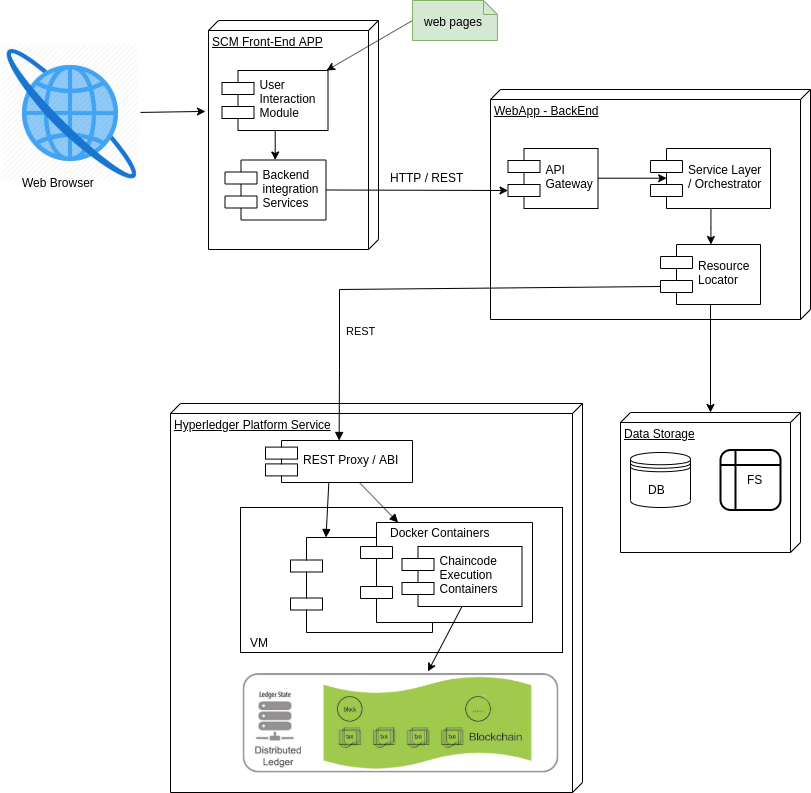
\includegraphics[scale=0.55]{images/detalhamentotecnico.png}
\caption{Application architecture of \ac{SCM-BP}}
\label{fig:detalhamentotecnico}
\end{center}
\end{figure}

\subsection{WebApp - FrondEnd}\label{sec:WebAppFrondEnd}
WebApp - FrontEnd is a client–server computer application which the client (including the user interface and client-side logic) runs in a web browser. This is a single-page application (SPA), a web application that interacts with the user by dynamically rewriting the current page rather than loading entire new pages from a server. This approach avoids interruption of the user experience between successive pages, making the application behave more like a desktop application.

The application is build with React (also known as React.js or ReactJS). This is a JavaScript library for building user interfaces. It is maintained by Facebook and a community of individual developers and companies. Used as a base in the development of single-page or mobile applications, React is optimal for fetching rapidly changing data that needs to be recorded. However, fetching data is only the beginning of what happens on a web page, which is why complex React applications usually require the use of additional libraries for state management, routing, and interaction with an API.

The Webapp - FrontEnd is divided into two main blocks and these are classified according to the interactions: User Interaction Modules and Backend Interactions Services.

\subsubsection{User Interaction}\label{sec:UserInteraction}
The User Interaction modules are responsible for providing web pages that will be rendered on client’s web browser. These interactions are provided by web pages grouped by the following modules:

\begin{itemize}
\item Login page
\item Application configuration module
\item User handling module (actors - CRUD)
\item Data entry module (forms)
\item Data visualization module
\item Reporting module
\end{itemize}

\subsubsubsection{Login Module}
The Login Module is responsible for display the login and authentication alternatives pages (‘forgot my password’, ‘reset my password’, etc.).

\subsubsubsection{Application configuration module}
The Application configuration module provides the features of creation/configuration of supply chain items and supply chain flows (steps and sub-tasks).

\subsubsubsection{User handling module}
This module provides the features for creation/configuration of Actors and Roles. The table in appendix \ref{app:userCreationFields} show the fields and values for creating a user.

\subsubsubsection{Data entry module}
The Data entry module provides form pages that allow users to enter data in the application, search and move assets from a step to another.

\subsubsubsection{Data visualization module}
The Data visualization module is responsible to display the information about assets in the supply chain flow. 

\subsubsubsection{Reporting Module}
In the Reporting module users can generate reports/files containing information organized in a narrative, graphic, or tabular form, prepared on ad hoc, periodic, recurring, regular, or as required basis. Reports may refer to specific periods, events, occurrences, or subjects, and may be presented in written form or any other format.

\subsubsection{Backend Interaction}\label{sec:BackendInteraction}
Backend interactions happen via a service layer consisting of:

\begin{itemize}
\item Authentication service
\item Application setup service
\item User creation service (actors)
\item Data entry service (forms)
\item Data visualization service
\item Reporting service
\end{itemize}

\subsubsubsection{Authentication Service}
The function of the Authentication Service is to request information from an authenticating party, and validate it against the configured identity repository using the specified authentication module. After successful authentication, the user session is activated and can be validated across all web applications participating in an SSO environment. For example, when a user or application attempts to access a protected resource, credentials are requested by one (or more) authentication modules. Gaining access to the resource requires that the user or application be allowed based on the submitted credentials.

\subsubsubsection{Application setup Service}
Application setup service provides methods to configure and edit  supply chain items and supply chain flows, defining which steps and sub-tasks will be present in this flow and which information will be present in these steps.

\subsubsubsection{User creation Service}
This service is responsible for the creation of users and roles, to allow them to log in and use the application’s features. Only Administrators are allowed to create new users (see Actions and Actors).

\subsubsubsection{Data entry Service}
Data entry service receives data from UI forms and send them to the backend to be processed and stored.

\subsubsubsection{Data visualization Service}
Data visualization services provides information about the supply chain: Assets, users and transactions, to be used by the data visualization module.

\subsubsubsection{Reporting Service}
Report services generate files (Doc/PDF/XSL, etc...) from a specific period of time with information about the supply chain: Assets, users and transactions.
\subsection{WebApp - BackEnd}\label{sec:WebAppBackEnd}
WebApp - BackEnd is a Middleware that runs on the server. This Middleware (server-side software) facilitates client-server connectivity, forming a middle layer between the app(s) and the network: the server, the database, the operating system, and more. It receives requests from the clients (in this case, the WebApp - FrontEnd), and contains the logic to send the appropriate data back to the applicant, over HTTP and REST.  These are the main conventions that provide structure to the request-response cycle between clients and servers.

WebApp - BackEnd is an application build with Node.js, an application platform where developers can write Javascript programs that are compiled, optimized and interpreted by the V8 virtual machine. Node.js can create quick, reliable websites and products in much efficient manner. Developing easy to scale real time applications in other technologies is bit difficult, but JavaScript technologies made it easier.

The WebApp - BackEnd is composed by the API Gateway, Service Layer and Resource Locator more detailed below.

\subsubsection{API Gateway}\label{sec:APIGateway}
API Gateway is a managed service that enables easily create, publish, maintain, monitor and secure REST APIs to act as a "gateway" for applications to access data, business logic, or functionality in the backend services, such as workloads. The API Gateway provides a simple uniform view of external resources to the internals of this application. It manages all tasks involved in receiving and processing API calls, including traffic management, authorization and access control, monitoring and management of API versions.

\begin{figure}[htbp]
\begin{center}
  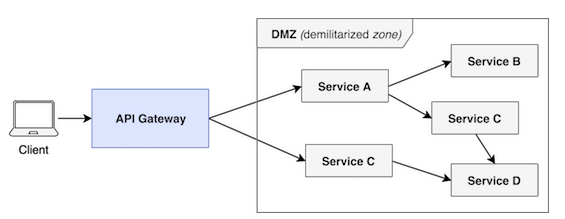
\includegraphics[scale=0.75]{images/apigateway.png}
\caption{API Gateway.}
\label{default-regular2}
\end{center}
\end{figure}

Basically, the Gateway is an interface that receives calls to its internal systems, being a large gateway. It act in five different ways:

\begin{itemize}
\item Filter for call traffic from different media;
\item Single gateway to the various APIs that are exposed;
\item Router: API and Rate Limit traffic router;
\item Security engine with authentication and logging.
\end{itemize}

Gateway access can be done from many different devices. Therefore, it must have the power to unify outgoing calls and be able to deliver to the user content that can be accessed from any browser and system. In this project the gateway interaction happens with the frontend webapp. The Gateways as a Security Feature: In the APIs world, one of the most subject talked about issues is always security, and having an API Gateway is one of the best solutions on the market to get full control of API’s, because this pattern addresses the so-called CIA (Confidentiality, Integrity, Availability) almost flawlessly.

\subsubsection{Service Layer}\label{sec:ServiceLayer}
A Service Layer defines an application's boundary and its set of available operations from the perspective of interfacing client layers. It encapsulates the application's business logic, controlling transactions and coordinating responses in the implementation of its operations.

Enterprise applications typically require different kinds of interfaces to the data they store and the logic they implement: data loaders, user interfaces, integration gateways, and others. Despite their different purposes, these interfaces often need common interactions with the application to access and manipulate its data and invoke its business logic. The interactions may be complex, involving transactions across multiple resources and the coordination of several responses to an action. Encoding the logic of the interactions separately in each interface causes a lot of duplication. the service layer provides:

\begin{enumerate}
\item Centralizes external access to data and functions.
\item Hides (abstracts) internal implementation and changes.
\item Allows for versioning of the services.
\end{enumerate}

The service layer acts as an orchestrator, controlling the flow of incoming and outcoming information requests and responses. Orchestration allows to directly link process logic to service interaction within workflow logic. This combines business process modeling with service-oriented modeling and design, realizing workflow management through a process service model. Orchestration brings the business process into the service layer, positioning it as a master composition controller.

\subsubsection{Resource Locator}\label{sec:ResourceLocator}

Resource locators are components that abstracts the persistence layer. Their job is to provide an object that can help services to discover and persist information from/to the Data Storage Module. Information can be stored in the Blockchain, Filesystem or Database and resource locators should know exactly where get/put data within them.  
\subsection{Data Storage}\label{sec:DataStorage}
Data storage is a general term for archiving data in electromagnetic or other forms for use by a computer or device. Different types of data storage play different roles in a computing environment. In addition to forms of hard data storage, there are now new options for remote data storage, such as cloud computing, and blockchain that can revolutionize the ways that users save and access data.  

SCM-BP uses three applications as data storages: Blockchain, Cloud filesystem and relational database better detailed on next subsections. Blockchains grow continuously because of the amount of data and code in them, which is unchanging. Therefore, an important design decision is to choose which data and calculations to keep in and out of the chain.

\subsubsection{Blockchain}\label{sec:DataStorageBlockchain}
A blockchain is a peer-to-peer distributed ledger forged by consensus, combined with a system for “smart contracts” and other assistive technologies. Together these can be used to build a new generation of transactional applications that establishes trust, accountability and transparency at their core, while streamlining business processes and legal constraints.

SCM-BP uses Blockchain as a supply chain that track parts and service provenance, ensure authenticity of goods, block counterfeits and reduce conflicts.

To achieve that, Hyperledger Fabric is used. Hyperledger is an open source collaborative effort created to advance cross-industry blockchain technologies. It is a global collaboration, hosted by The Linux Foundation, including leaders in finance, banking, Internet of Things, supply chains, manufacturing and Technology.
Hyperledger Fabric is an enterprise-grade permissioned distributed ledger framework for developing solutions and applications. Its modular and versatile design satisfies a broad range of industry use cases. It offers a unique approach to consensus that enables performance at scale while preserving privacy.

In context of SCM-BP, the Blockchain module consists in a smart contract, chaincode and the ledger. From the application developer’s perspective, a smart contract, together with the ledger, form the heart of a Hyperledger Fabric blockchain system. Whereas a ledger holds facts about the current and historical state of a set of business objects, a smart contract defines the executable logic that generates new facts that are added to the ledger. A chaincode is typically used by administrators to group related smart contracts for deployment, but can also be used for low level system programming of Fabric.

\subsubsubsection{Smart contract}
Before businesses can transact with each other, they must define a common set of contracts covering common terms, data, rules, concept definitions, and processes. Taken together, these contracts lay out the business model that govern all of the interactions between transacting parties.

A smart contract defines the rules between different organizations in executable code. Applications invoke a smart contract to generate transactions that are recorded on the ledger.

\subsubsubsection{Chaincode}
Hyperledger Fabric users often use the terms smart contract and chaincode interchangeably. In general, a smart contract defines the transaction logic that controls the lifecycle of a business object contained in the world state. It is then packaged into a chaincode which is then deployed to a blockchain network. Think of smart contracts as governing transactions, whereas chaincode governs how smart contracts are packaged for deployment.

\subsubsubsection{Ledger}
At the simplest level, a blockchain immutably records transactions which update states in a ledger. A smart contract programmatically accesses two distinct pieces of the ledger – a blockchain, which immutably records the history of all transactions, and a world state that holds a cache of the current value of these states, as it’s the current value of an object that is usually required.

Smart contracts primarily put, get and delete states in the world state, and can also query the immutable blockchain record of transactions.

\begin{itemize}
\item A \textbf{get} typically represents a query to retrieve information about the current state of a business object.
\item A \textbf{put} typically creates a new business object or modifies an existing one in the ledger world state.
\item A \textbf{delete} typically represents the removal of a business object from the current state of the ledger, but not its history.
\end{itemize}

Smart contracts have many APIs available to them. Critically, in all cases, whether transactions create, read, update or delete business objects in the world state, the blockchain contains an immutable record of these changes.

\subsubsection{Filesystem}\label{sec:Filesystem}
A cloud file system is a tiered storage system that provides shared access to file data. Users can create, delete, modify, read and write files, as well as logically organize them into directory trees for intuitive access.

Cloud file sharing can be defined as a service that gives multiple users simultaneous access to a cloud file data set. Cloud file sharing security is managed with user and group permissions, allowing administrators to tightly control access to shared file data.

For all file uploaded and stored in the filesystem, a locally stored digital fingerprint (hash) is saved in the blockchain, separately from the original files or content, to make it easier to confirm whether data has been altered or manipulated in a particular organization.

\subsubsection{Database}\label{sec:Database}
A relational database is a set of formally described tables from which data can be accessed or reassembled in many different ways without having to reorganize the database tables. The standard user and application programming interface (API) of a relational database is the Structured Query Language (SQL). SQL statements are used both for interactive queries for information from a relational database and for gathering data for reports.

\section{Actions And Actors}\label{sec:actionsAndActors}

A set of rules governs the system. These rules define how users interact with the system and how the data is shared among the users. Moreover, once the rules are stored in the blockchain, they can not be altered without broadcasting to all nodes and verified by most of them.
%%% SETUP

\subsection{Setup}\label{sec:Setup}
Setup is the set of actions to configure the application. The setup phase is when a new supply chain is created, or an existing one is updated or deleted. Users can also be created, updated, and deleted by setup actions. When creating or editing a supply chain, Admin users will define which steps, sub-steps, and information the supply chain flow will contain. Users from member groups can add info and move an asset to each step in the logistics network.

Administrators are the only users in the Admin group. This actor type has access to all areas of the program. It has the same abilities like all other user types (configuring, moving the asset, and viewing flow). However, his primary responsibility is to configure the application and perform the setup actions.


%%% DATA INSERTION

\subsection{Data Insertion}\label{sec:DataInsertion}

Data insertion is the action that will fill the supply chain flow with data. Once the admin user creates a new supply chain, it is ready to be populated with information. Member and admin users are responsible for performing these actions. In the Data Insertion phase, users can update information from a specific step and sub-step and move assets depending on the rules applied in the setup phase. The most common actor types in SCM are Raw material/Producer, Manufacturer, Distributor Wholesaler, and Retailer.

%%% VISUALIZATION

\subsection{Visualization}\label{sec:Visualization}

Any user in the system can perform visualization actions. However, its main purpose is to provide the end-user the capability to track the flow of an asset from the point of origin to the point of consumption.
\section{Implementation Details}\label{sec:Implementation}

The chaincode is written in Golang and provides all contracts needed to proceed traceability in the application. All contracts for use in chaincode must implement the interface \textit{contractapi.ContractInterface}. 

The first step is to create a JSON config file providing all information about these three items. A configuration file includes \textit{assetId}, a list of actors and a list of ordered steps. The chaincode processes this file through  \textit{initLedger} and \textit{createNewAsset} functions. Here follows a template for config file:  

\begin{minted}{json}
{
   "AssetId":"assetID",
   "AssetName":"assetName",
   "AssetDescription":"assetDescription",
   "Actors":[
      {
         "actorType":"type",
         "aditionalInfo":[
            {
               "key":"value"
            }
         ]
      }
   ],
   "Steps":[
      {
         "StepId":"stepID",
         "StepName":"stepName",
         "StepOrder":1,
         "ActorType":"actorType",
         "aditionalInfo":[
            {
               "key":"value"
            }
         ]
      }
   ]
}
\end{minted}

Front-end WebApp enables a user to define settings through a Configuration Page, adding these to the configuration file, as shown in Figure~\ref{fig:create_asset_4}.

Assets, asset items, steps and actors are described as \textit{structs}, as follows:

\begin{minted}{go}
type Actor struct {
  ActorId    string  `json:"actorId"`
  ActorType  string  `json:"actorType"`
  ActorName  string  `json:"actorName"`
  Deleted    bool    `json:"deleted"`
  AditionalInfo map[string]string `json:"  aditionalInfo"`
}

type Step struct {
  StepId     string  `json:"stepId"`
  StepName   string  `json:"stepName"`
  StepOrder  uint    `json:"stepOrder"`
  ActorType  string  `json:"actorType"`
  Deleted    bool    `json:"deleted"`
  AditionalInfo map[string]string `json:"  aditionalInfo"`
}

type AssetItem struct {
  AssetItemId   string    `json:"assetItemId"`
  OwnerId       string    `json:"ownerId"`
  StepID        string    `json:"stepID"`
  ParentID      string    `json:"parentID"`
  Children      []string  `json:"children"`;
  ProcessDate   string    `json:"processDate"`
  DeliveryDate  string    `json:"deliveryDate"`
  OrderPrice    string    `json:"orderPrice"`
  ShippingPrice string    `json:"shippingPrice"`
  Status        string    `json:"status"`
  Quantity      string    `json:"quantity"`
  Deleted       bool      `json:"deleted"`
  AditionalInfo map[string]string `json:"  aditionalInfo"`
}

type Asset struct {
  AssetId      string       `json:"assetId"`
  AssetName    string       `json:"assetName"`
  Description  string       `json:"description"`
  AssetItems   []AssetItem  `json:"assetItems"`
  Actors       []Actor      `json:"actors"`
  Steps        []Step       `json:"steps"`
  Deleted      bool         `json:"deleted"`
  AditionalInfo map[string]string `json:"aditionalInfo"`
}
\end{minted}

There are create methods for each one,  responsible for creating an instance of these \textit{structs} and save the state into the Blockchain. Query methods are responsible for interact with the information of any item in the Blockchain.


The chaincode \textit{main} function invokes the \textit{initLedger} function, reads the configuration files and raises the platform enabling users to interact with the Blockchain via exposing its API, as follows: 

\begin{minted}{go}
func main() {
  chaincode, err := contractapi.NewChaincode(new(SmartContract))
  if err != nil {
    fmt.Printf("Error create chaincode: %s", err.Error())
    return
  }
  if err := chaincode.Start(); err != nil {
    fmt.Printf("Error starting chaincode: %s", err.Error())
  }
}
\end{minted}

When creating an asset item, an \textit{AssetItemId} is generated. Each entity in the chain will have its unique entity ID and timestamp when it starts processing the transaction. By querying \textit{AssetItemId}, the user can easily track the current transaction information and status. Finally, completed all steps, the Blockchain will update \textit{deliverDate} and mark the status as completed once the last actor (generally the consumer) has received the order. Here follows \textit{CreateAsset} function:

\begin{minted}{go}
func (s *SmartContract) CreateAsset(
  ctx contractapi.TransactionContextInterface, assetId string,
  assetName string, description string, assetItems []AssetItem, 
  actors []Actor, steps []Step, aditionalInfo map[string]string) error {
  
  if err != nil {
    return fmt.Errorf(
      "Failed to read the data from world state: %s", err
    )
  }

  if assetJSON != nil {
    return fmt.Errorf("The asset %s already exists", assetID)
  }
  
  asset := Asset {
    AssetId:       assetId,
    AssetName:     assetName,
    Description:   description,
    AssetItems:    assetItems,
    Actors:        actors,
    Steps:         steps,
    Deleted:       false,
    aditionalInfo: aditionalInfo,
  }
  assetAsBytes, _ := json.Marshal(asset)
  if err != nil {
    return err
  }
  return ctx.GetStub().PutState("ASSET_"+assetId,assetAsBytes)
}
\end{minted}

\textit{MoveAssetItem} is the method called to update an asset item when it is moved from a step to another. It updates the \textit{CurrentOwnerId}, the \textit{ProcessDate}, information about prices and many other details of the transactions by the key/value map \textit{  aditionalInfo}. Here follows this fuction:

\begin{minted}{go}
func (s *SmartContract) MoveAssetItem(
  ctx contractapi.TransactionContextInterface, 
  assetItemID string, newAssetItemID string, stepID string, 
  newOwnerID string, orderPrice string, shippingPrice string, 
  status string, quantity string, 
  aditionalInfo map[string]string ) error {
  
  assetItemJSON, err := s.QueryAssetItem(ctx, assetItemID)
  if err != nil {
    return err
  }
  if assetItemJSON == nil {
    return fmt.Errorf("The assetItem %s does not exists", assetItemID)
  }

  newAssetItem := AssetItem{
    AssetItemID:      newAssetItemID,
    OwnerID:          newOwnerID,
    StepID:           stepID,
    ParentID:         assetItemID,
    Children:         []string{},
    ProcessDate:      time.Now().Format("2006-01-02 15:04:05"),
    OrderPrice:       orderPrice,
    ShippingPrice:    shippingPrice,
    Status:           status,
    Quantity:         quantity,
    Deleted:          false,
    AditionalInfoMap: aditionalInfo,
  }

  assetItemAsBytes, err := json.Marshal(newAssetItem)
  if err != nil {
    return err
  }

  return ctx.GetStub().PutState(
    "ASSET_ITEM_"+newAssetItemID, assetItemAsBytes
  )
}
\end{minted}

\textit{TrackAssetItem} is the method responsible for track an asset item. It returns the children tree of the given element and its ancestors from the beginning of the Supply chain. This method uses the function getChildenTree to get the current item's children nodes: 

\begin{minted}{go}
func (s *AssetTransferSmartContract) TrackAssetItem(
  ctx contractapi.TransactionContextInterface, 
  assetItemID string) ([]*AssetItem, error) {
  
  assetItem, err := s.QueryAssetItem(ctx, assetItemID)
  log.Print("tracking info from assetItem id: ", assetItem.AssetItemID)
  if err != nil {
    return nil, fmt.Errorf(
      "Failed to read from world state. %s", err.Error()
    )
  }

  if assetItem == nil {
    return nil, fmt.Errorf("%s does not exist", assetItemID)
  }

  trackedItems := make([]*AssetItem, 0)

  //first add the children to tracked items
  children, err := s.getChildenTree(ctx, assetItem)
  if err != nil {
    return nil, fmt.Errorf(
      "Failed to read from world state. %s", err.Error()
    )
  }

  for _, child := range children {
    fmt.Println(child)
    trackedItems = append(trackedItems, child)
  }

  //then, add the current item to tracked items
  trackedItems = append(trackedItems, assetItem)

  //finally, add the ancestor of current item to tracked items
  for {
    currentParentId, err := strconv.Atoi(assetItem.ParentID)
    if (currentParentId <= 0) {
      break
    }
    parentAssetItem, err := s.QueryAssetItem(ctx, assetItem.ParentID)
    if err != nil {
      return nil, fmt.Errorf(
        "Failed to read from world state. %s", err.Error()
      )
    }
    newParentId, err := strconv.Atoi(parentAssetItem.ParentID)
    log.Print("newParentId: ", newParentId)
    trackedItems = append(trackedItems, parentAssetItem)
    assetItem = parentAssetItem
  }
  return trackedItems, nil
}

func (s *AssetTransferSmartContract) getChildenTree(
  ctx contractapi.TransactionContextInterface, 
  assetItem *AssetItem) ([]*AssetItem, error) {
  
  tree := make([]*AssetItem, 0)
  log.Print("len(assetItem.Children): ", len(assetItem.Children))
  if len(assetItem.Children) == 0 {
    tree = append(tree, assetItem)
  } else {
    for _, childId := range assetItem.Children {
      childAssetItem, err := s.QueryAssetItem(ctx, childId)
      if err != nil {
        return nil, fmt.Errorf(
          "Failed to read from world state. %s", err.Error()
        )
      }
      if childAssetItem == nil {
        return nil, fmt.Errorf("%s does not exist", childId)
      }

      childrenTree, err := s.getChildenTree(ctx, childAssetItem)
      for _, child := range childrenTree {
        tree = append(tree, child)
      }
    }
    tree = append(tree, assetItem)
  }
  return tree, nil
}
\end{minted}


Figure~\ref{fig:sequenceDiagram} shows the interaction flow from users with Árion platform. Initially, an admin persona creates and configure the SCM, adding information about the steps and the users. After that, the admin can activate this SCM, and from that point, the actors can interact with the SCM to provide information about an asset item and also move this asset item through the supply chain. From that point too, any user can track an asset item to get information about the required good.

%htbp
\begin{figure}[ht]
\begin{center}
  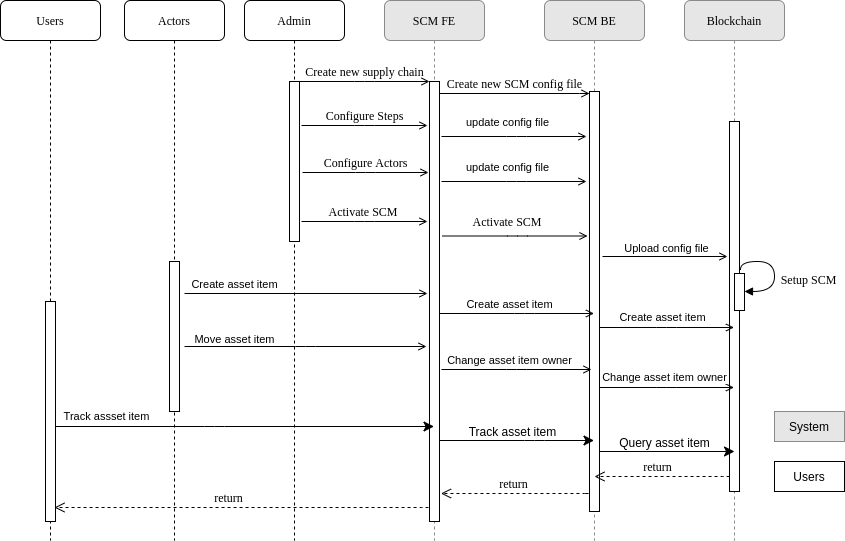
\includegraphics[scale=0.5]{images/SequenceDiagram.png}
\caption{SCM User flow}
\label{fig:sequenceDiagram}
\end{center}
\end{figure}


The backend gateway exposes all the endpoints shown in table \ref{table:endpoints}. These endpoints are integrated with the frontend and can be used in the future work to integrate with a mobile app or an external application.


\begin{table}[htb]
\centering
\caption{Backend endpoints}
\label{table:endpoints}
    \begin{center}
    \begin{tabular}{|l|p{4.5cm}|p{7.664cm}|}
        \hline 
        \thead{Verb} & \thead{URI} & \thead{Description}\\
        \hline 
        \cellcolor{cyan}\textbf{Actors}  & \cellcolor{cyan}\textbf{} & \cellcolor{cyan}\textbf{} \\
        \hline 
        POST & /actors & creates a new actor\\
        \hline 
        GET & /actors & retrieves the actors' list\\
        \hline 
        PUT & /actors/:id & updates an existing actor\\
        \hline 
        GET & /actors/:id & retrieves an existing actor\\
        \hline 
        DELETE & /actors/:id & removes an existing actor\\
        \hline 
        \cellcolor{cyan}\textbf{Steps}  & \cellcolor{cyan}\textbf{} & \cellcolor{cyan}\textbf{} \\
        \hline 
        POST & /steps & creates a new step\\
        \hline 
        GET & /steps & retrieves the steps' list\\
        \hline 
        PUT & /steps/:id & updates an existing step\\
        \hline 
        GET & /steps/:id & retrieves an existing step\\
        \hline 
        DELETE & /steps/:id & removes an existing step\\
        \hline 
        \cellcolor{cyan}\textbf{Asset Items}  & \cellcolor{cyan}\textbf{} & \cellcolor{cyan}\textbf{} \\
        \hline 
        POST & /asset-items & creates a new asset item\\
        \hline 
        GET & /asset-items & retrieves the asset items' list\\
        \hline 
        PUT & /asset-items/:id & updates an existing asset item\\
        \hline 
        GET & /asset-items/:id & retrieves an existing asset item\\
        \hline 
        DELETE & /asset-items/:id & removes an existing asset item\\
        \hline 
        POST & /asset-items/:id & moves an asset item through the SCM\\
        \hline 
        GET & /asset-items/track/:id & tracks an asset item through the SCM\\
        \hline
        \cellcolor{cyan}\textbf{Assets}  & \cellcolor{cyan}\textbf{} & \cellcolor{cyan}\textbf{} \\
        \hline 
        POST & /assets & creates a new asset\\
        \hline 
        GET & /assets & retrieves the assets' list\\
        \hline 
        PUT & /assets/:id & updates an existing asset\\
        \hline 
        GET & /assets/:id & retrieves an existing asset\\
        \hline 
        DELETE & /assets/:id & removes an existing asset\\
        \hline 
    \end{tabular}
    \end{center}
\end{table}

%\xchapter{Proof of Concept}{} %sem preambulo
%\label{chap:useExample}

\acresetall 

\section{Proof of Concept}\label{sec:method}

For this project development, the agile Scrum method has been used. In Scrum, projects are divided into cycles called sprints, with frequent meetings where the team can inform what is being done and think of ways to improve the process quickly. Scrum proposes constant project monitoring. Often the team will be meeting, exchanging experiences, evaluating what has been done, and re-planning what will be done next.

During the requirements gathering, developers and other stakeholders sought to raise and prioritize the needs of future software users (referred to as requirements). After the requirements gathering, in the requirements specification stage, developers made a detailed study of data collected in the previous activity, from where models were built to represent the software system being developed.

At the architectural design stage of the system, two basic activities were performed: architectural design (or high-level design) and detailed design (or low-level design). Some aspects were considered at this stage of system design, such as system architecture, the platform used, Database Manager System (DBMS) used, and graphical interface standard.

In the application development period, the backend and frontend components were created from the computational description of the design phase. Pre-existing software tools and class libraries were used to streamline activity. These tools and libraries were defined during the architectural design and were referenced in \cref{sec:WebAppFrondEnd,sec:WebAppBackEnd}.

For system validation, two main requirements were evaluated: the components and the behavior of who will use the application. For the first point, functional, integration, and security tests will be performed. For the second, this proof of concept was applied.

Appendix \ref{app:projectManagement} presents the activities for project management, the user stories, and non-functional requirements. 


\section{Use Example}\label{sec:workflow}

To accomplish this usage example, one Coffee supply chain will be defined and configured accordingly. The supply chain of coffee beans is a lengthy process that involves growing the beans, harvesting, hulling, drying, packing, bulking, blending, and finally roasting. In between this process, the beans go through international transporters, export sellers, and retailers like grocery stores, cafes, and specialty shops. A coffee tree can take four to seven years before it yields its first crop of beans. The harvesting process is a very labor-intensive exercise. Parts of the cherry must be removed to access the beans and need to be laid out to dry. Once the beans are dried, they are packaged into large sacks and passed onto the exporters. They are distributed to big companies in the coffee business who take these beans and put them in industrial roasting and distribution centers. The inventory stock from the roasting and distributing centers must be passed forward to retailers. Through a web of transport, these coffee beans are delivered to thousands of roasters, cafes, restaurants, grocery stores, and large chain retailers, where they finally will come to the final users who will taste its flavor. 

For this scenario, five steps will be taken: Extraction is the step where the coffee is growing and picking. Processing is when the beans are dry, roasting, grinding, and packaging. Distribution is when the packages are shipping. Retail is about selling the product, and the final step is the final user consumption.

Five fictitious business enterprises and a final customer are named as follows: Tasty Coffee Farm, situated in Brazil, is an extractor responsible for all the information regarding the extraction step in the supply chain. Café Brazilium is the manufacturer and is responsible for the processing step. There will be two distribution companies. The first is Edgard Cargo which is the Distributor company and is in charge of distribution details. This company will send the coffee produced in Brazil to the United States. The second is O'Neil DistInc, a competitor of the first one. Marques BigSales is a United States situated Delicatessen store and is at the helm of selling details. Allan Manoel Jr. is a customer who wants to experiment with Brazilian coffee for the first time. Being very curious, the customer would like to know the provenance and the information about the coffee he drinks and where the coffee has passed.

As actors, each company above will have one user configured in the platform:  

\begin{itemize}
\item Extractor: James Johnson.
\item Manufacturer: Donald Jackson.
\item Distribution: Elizabeth Taylor.
\item Distribution: Charlotte O'Neil.
\item Retailer: BigSales.
\item Customer: Allan Manoel Jr.
\end{itemize}

The first step when creating a new Supply Chain  is to create and configure the asset. The admin user makes this action. By going through the setup wizard, first, the asset's info is requested:

\begin{figure}[H]
\begin{center}
  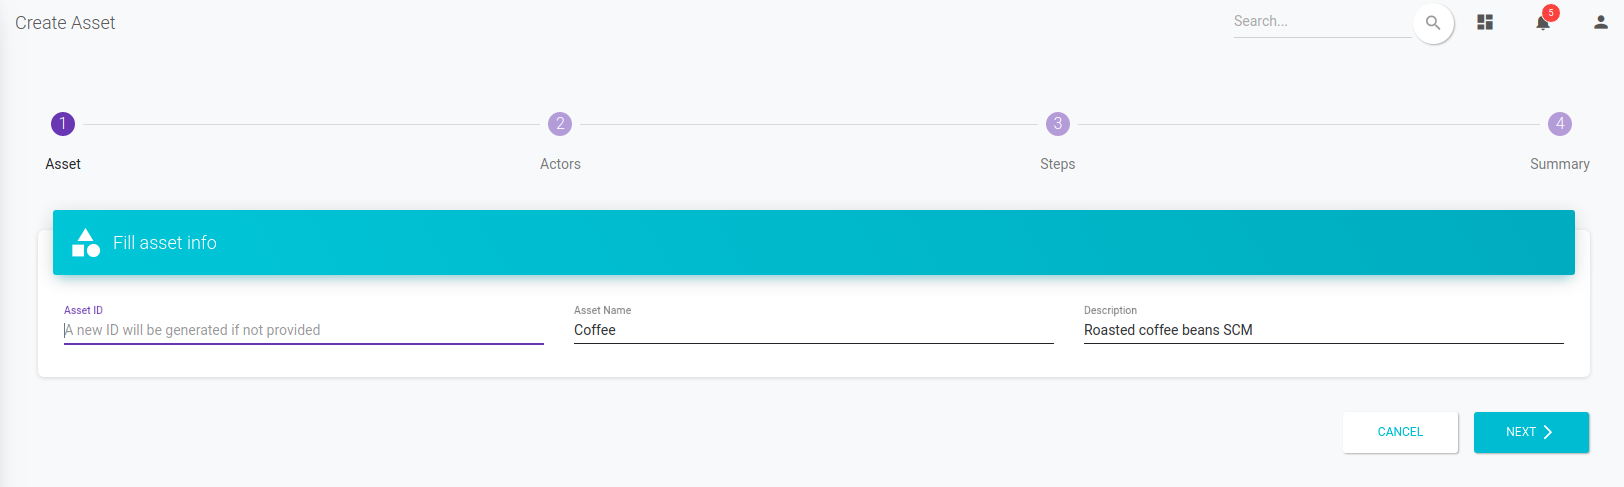
\includegraphics[scale=0.27]{images/use_example/01_create_asset_1.png}
\caption{Fill in asset info.}
\label{fig:create_asset_1}
\end{center}
\end{figure}

Then the admin will add actors to the SCM, informing its types. Actors can be added, updated, or deleted later on the actors' list page.

\begin{figure}[H]
\begin{center}
  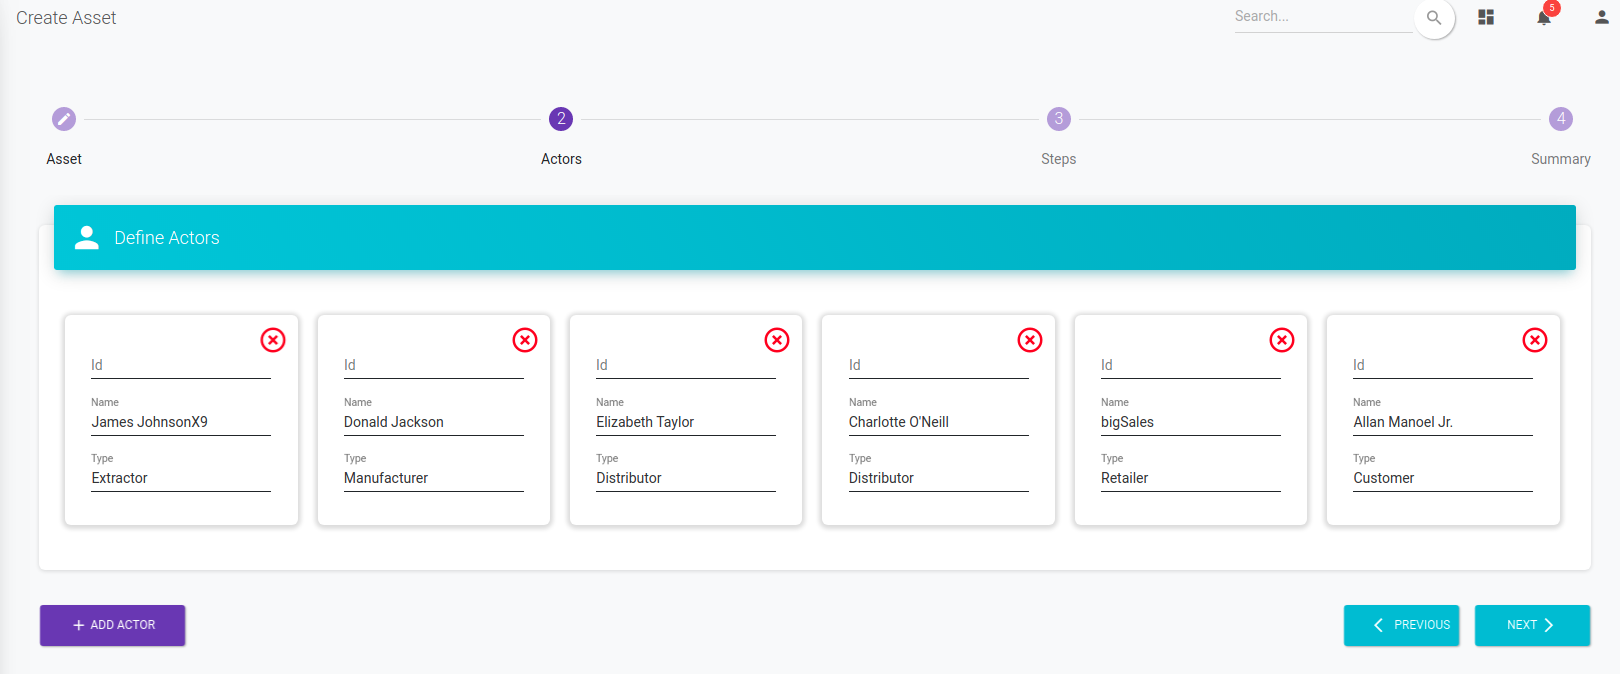
\includegraphics[scale=0.27]{images/use_example/02_create_asset_2.png}
\caption{Adding actors.}
\label{fig:create_asset_2}
\end{center}
\end{figure}


The next phase in the wizard is to define the Supply chain steps, specifying the order and binding it to the previous created actors' types:

\begin{figure}[H]
\begin{center}
  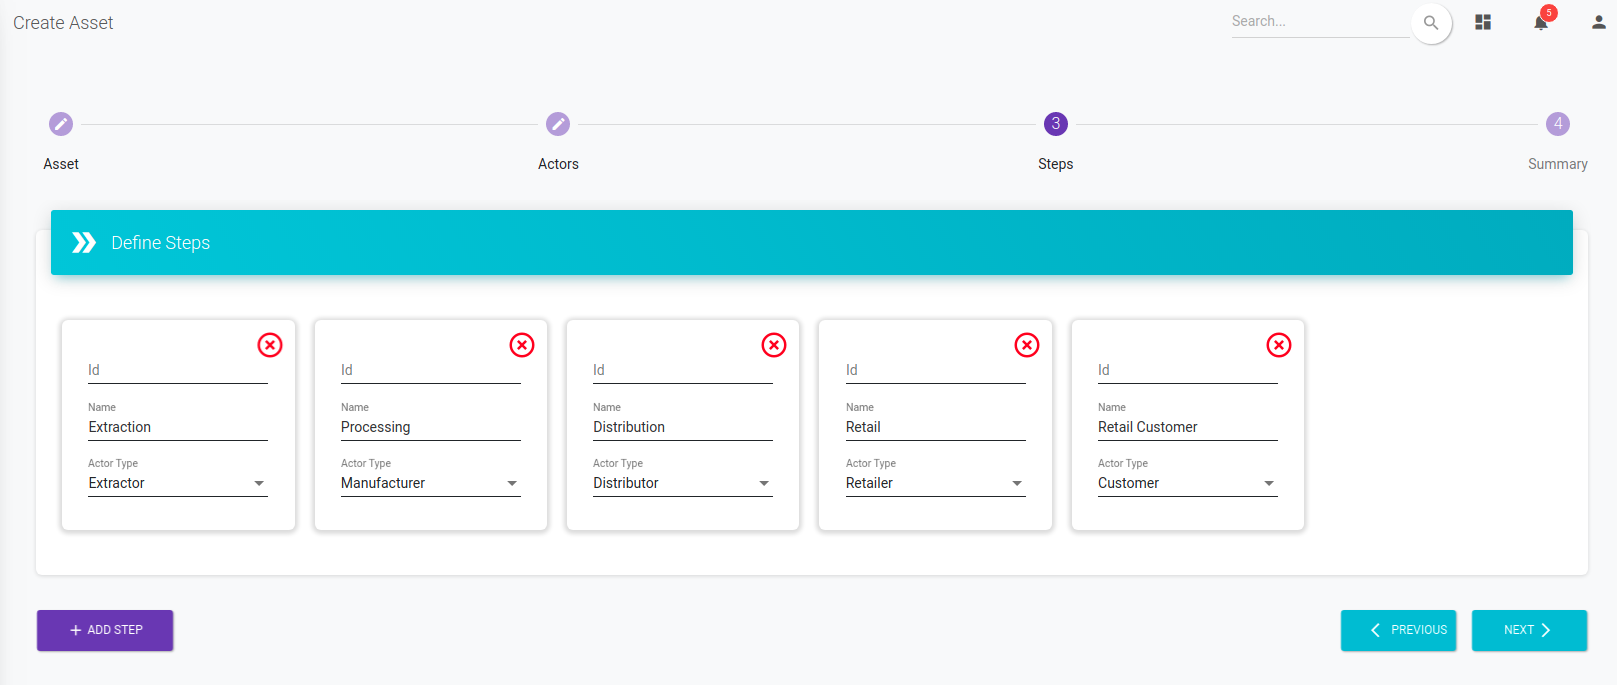
\includegraphics[scale=0.27]{images/use_example/03_create_asset_3.png}
\caption{Defining steps.}
\label{fig:create_asset_3}
\end{center}
\end{figure}

The final step, before submitting the form, is to review all the information previously added in the review asset details page, under the wizard:
\begin{figure}[H]
\begin{center}
  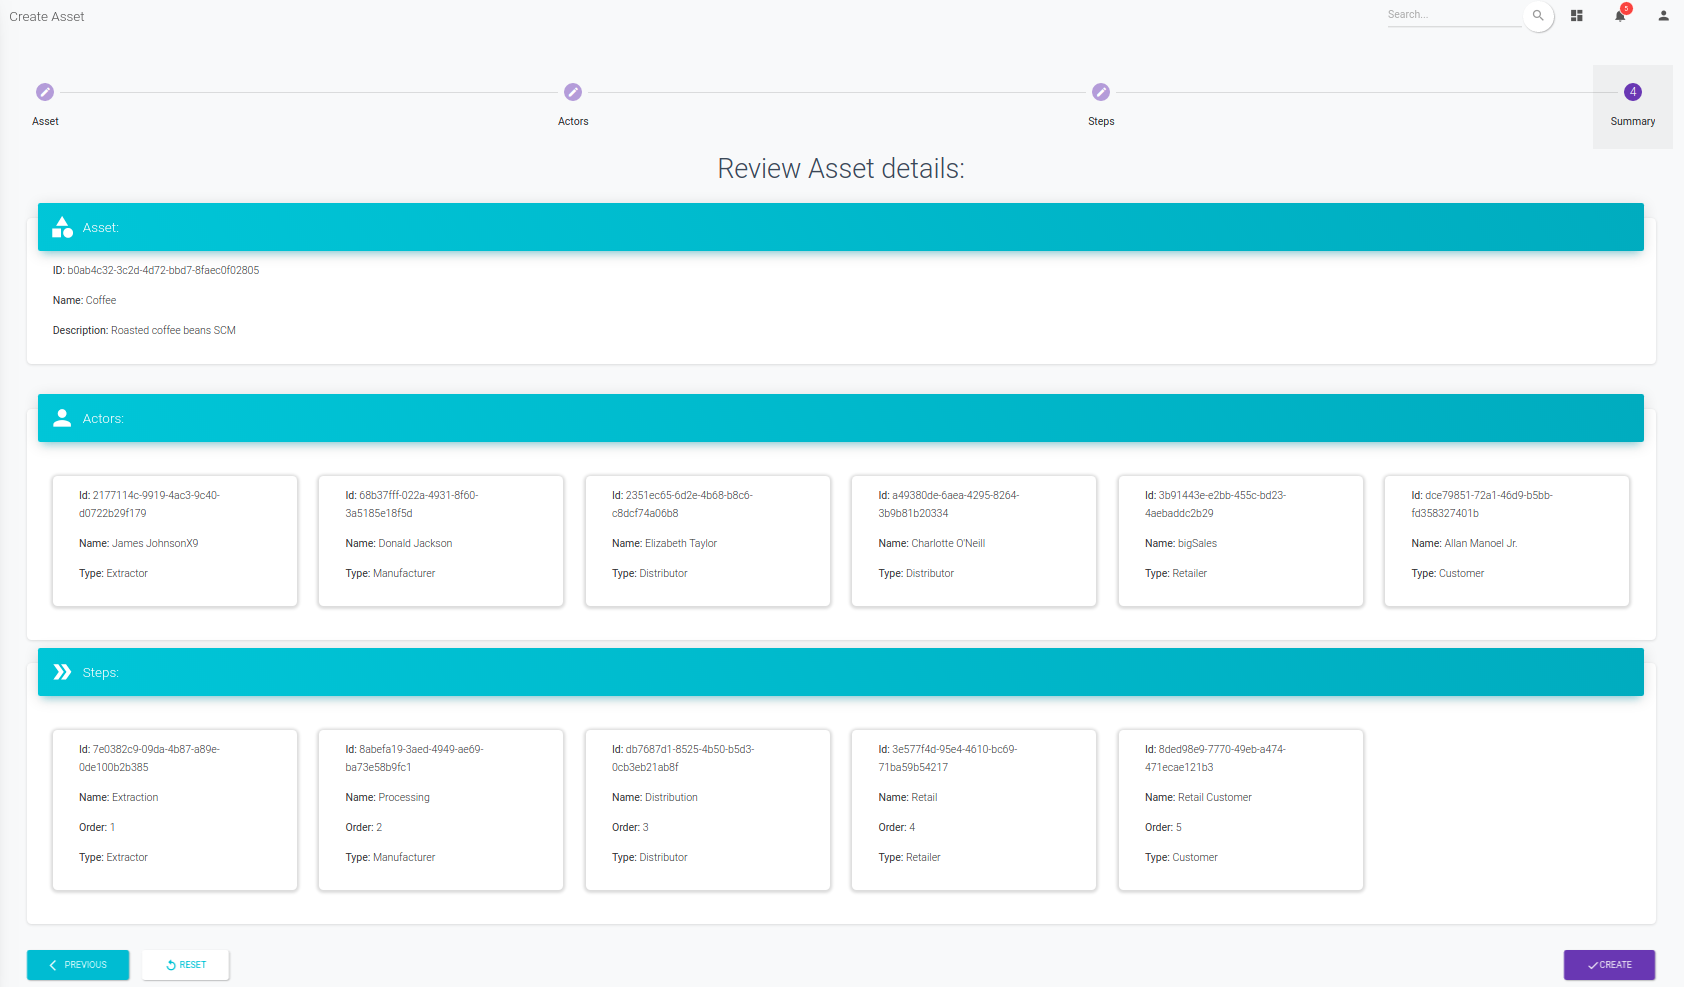
\includegraphics[scale=0.265]{images/use_example/04_create_asset_4.png}
\caption{Review asset details before submitting.}
\label{fig:create_asset_4}
\end{center}
\end{figure}


Once created, the asset can be seen in the assets list, where the admin can perform crud operations by the actions items. When clicking in the asset details, the current user is redirected to the asset details page, where the main information about asset items.
%, actors and steps can be seen. The card header contains a tab menu to provide navigation through these entities. 



% \begin{figure}[H]
% \begin{center}
%   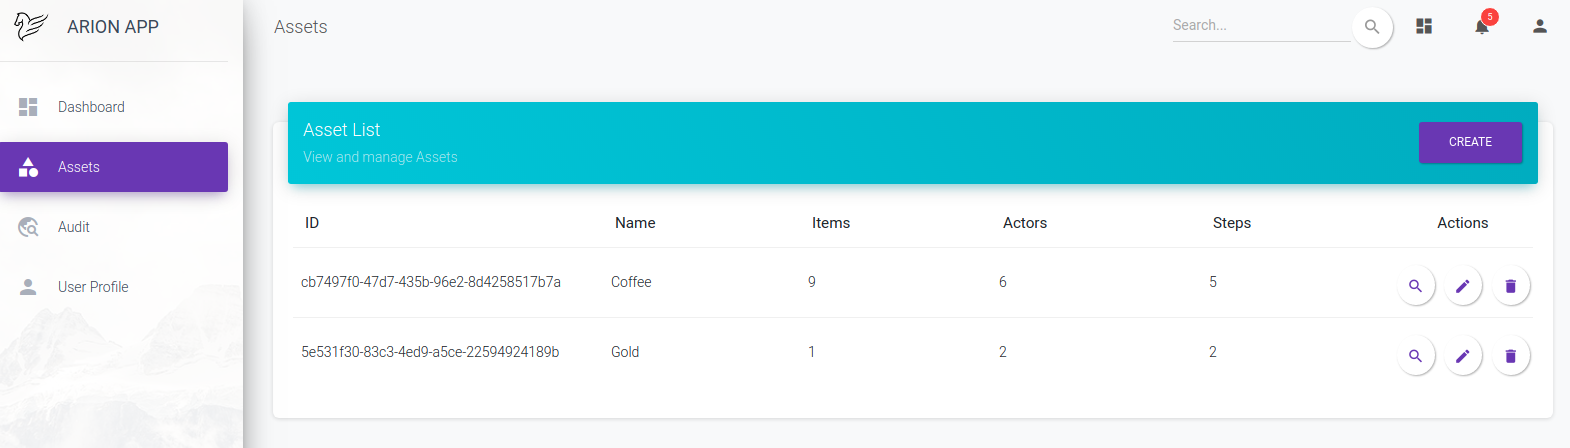
\includegraphics[scale=0.28]{images/use_example/05_asset_list.png}
% \caption{Asset list and action buttons.}
% \label{fig:asset_list}
% \end{center}
% \end{figure}



\begin{figure}[H]
\setlength{\belowcaptionskip}{-10pt}
\begin{center}
  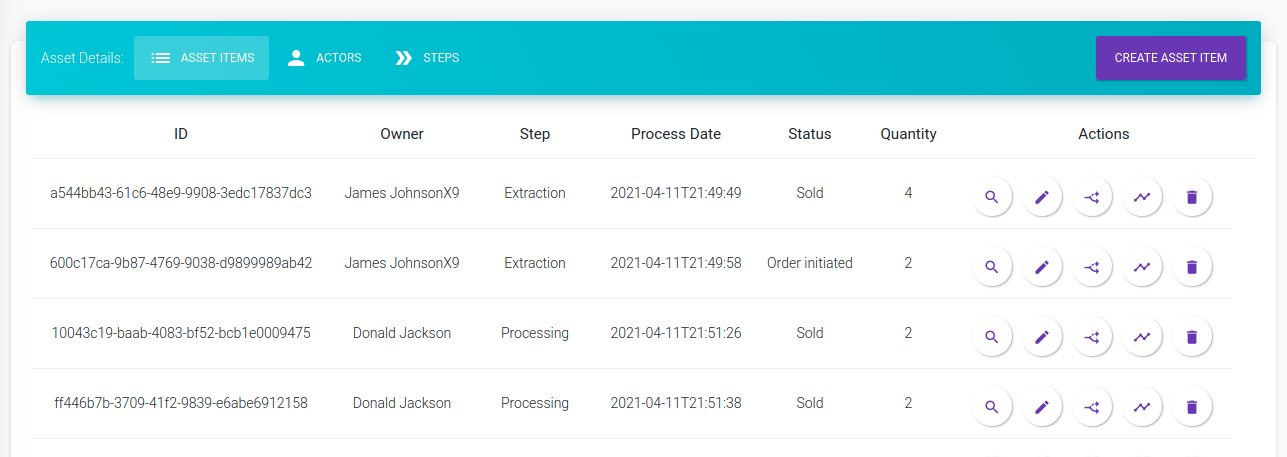
\includegraphics[scale=0.35]{images/use_example/06_asset_Item_list.png}
\caption{Asset Items list.}
\label{fig:asset_item_list}
\end{center}
\end{figure}

\begin{figure}[H]
\begin{center}
  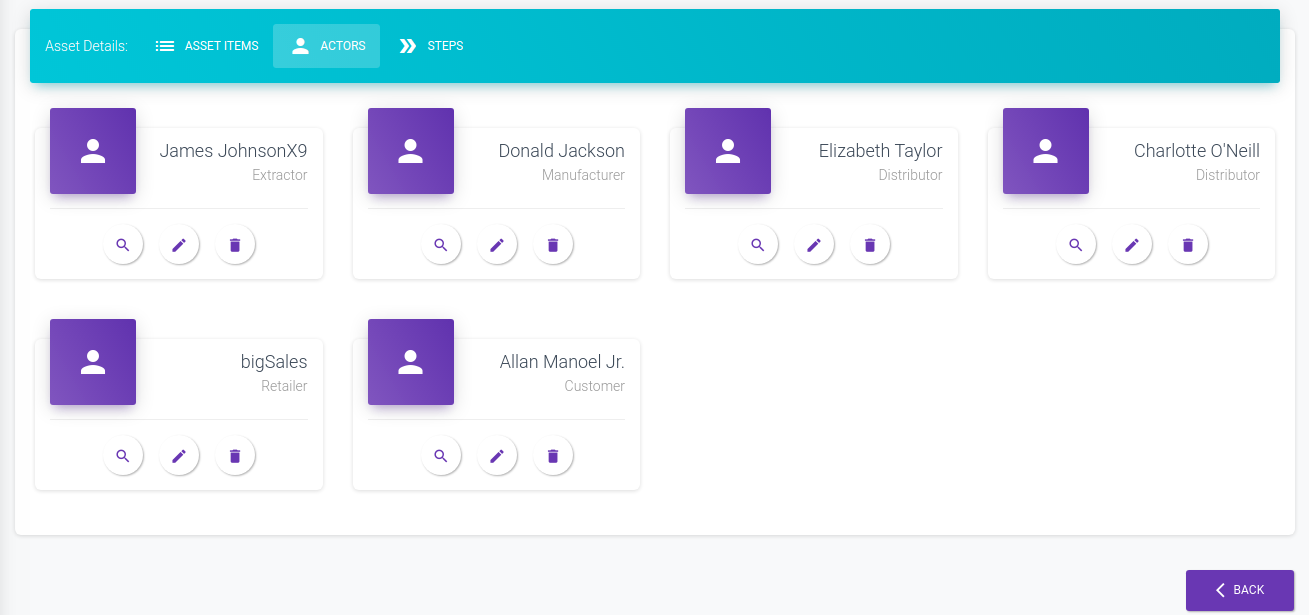
\includegraphics[scale=0.34]{images/use_example/07_actor_list.png}
\caption{Actors list.}
\label{fig:actor_list}
\end{center}
\end{figure}

\begin{figure}[H]
\begin{center}
  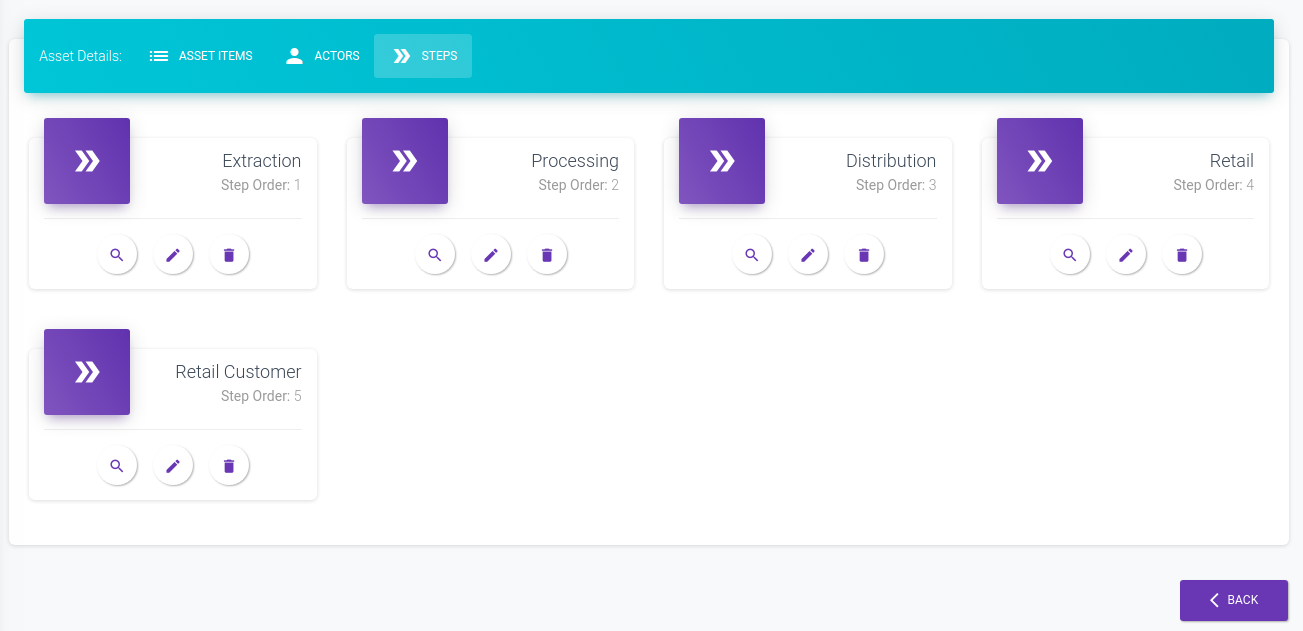
\includegraphics[scale=0.32]{images/use_example/08_steps_list.png}
\caption{Steps list.}
\label{fig:step_list}
\end{center}
\end{figure}

As an admin, there are also button actions to perform crud operations. Beyond Admins, actors responsible for the first step are allowed to create an asset item. This action will redirect the user to the create asset item form shown below. In the use case, a coffee crop was harvested by the extraction company. Information about this step is added at this point. 

\begin{figure}[H]
\begin{center}
  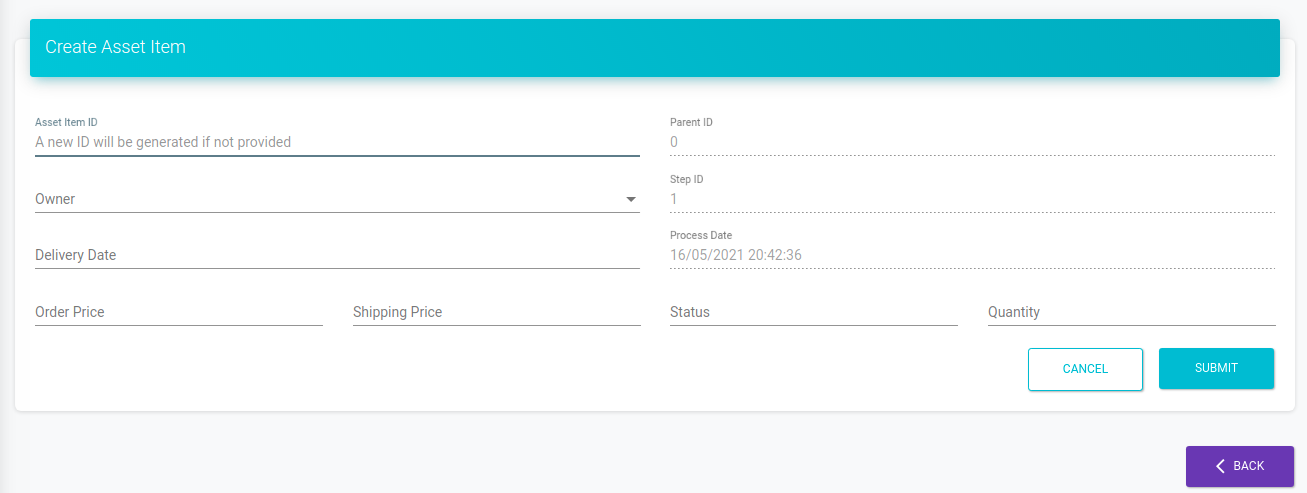
\includegraphics[scale=0.3]{images/use_example/09_create_asset_Item.png}
\caption{Create asset item form.}
\label{fig:create_asset_item}
\end{center}
\end{figure}


Beyond the crud actions in the asset items list, there are also two new actions: move asset item and track asset item. The first one shows a form where the user can move an asset through the SCM steps. The user can only move this asset item to the next or the previous step in the supply chain. Move an item back to the previous step is a feature that can be used when a customer needs to return the product to whoever sold it, for example, when a product comes defective, or the customer wants to exchange it. 

To the use case, the companies are using this feature to move towards the products. First, the Manufacturer company bought two lots from the same coffee crop of the extraction company. The manufacturer sold them into three lots after processing the products. The first and the second one were sent to the first distributor company and the third to the second distributor. The first distributor delivered the first lot to the retail company, and from this lot, a cup of coffee was sold to the final customer. All these actions were made from the moving asset item form below:

\begin{figure}[H]
\begin{center}
  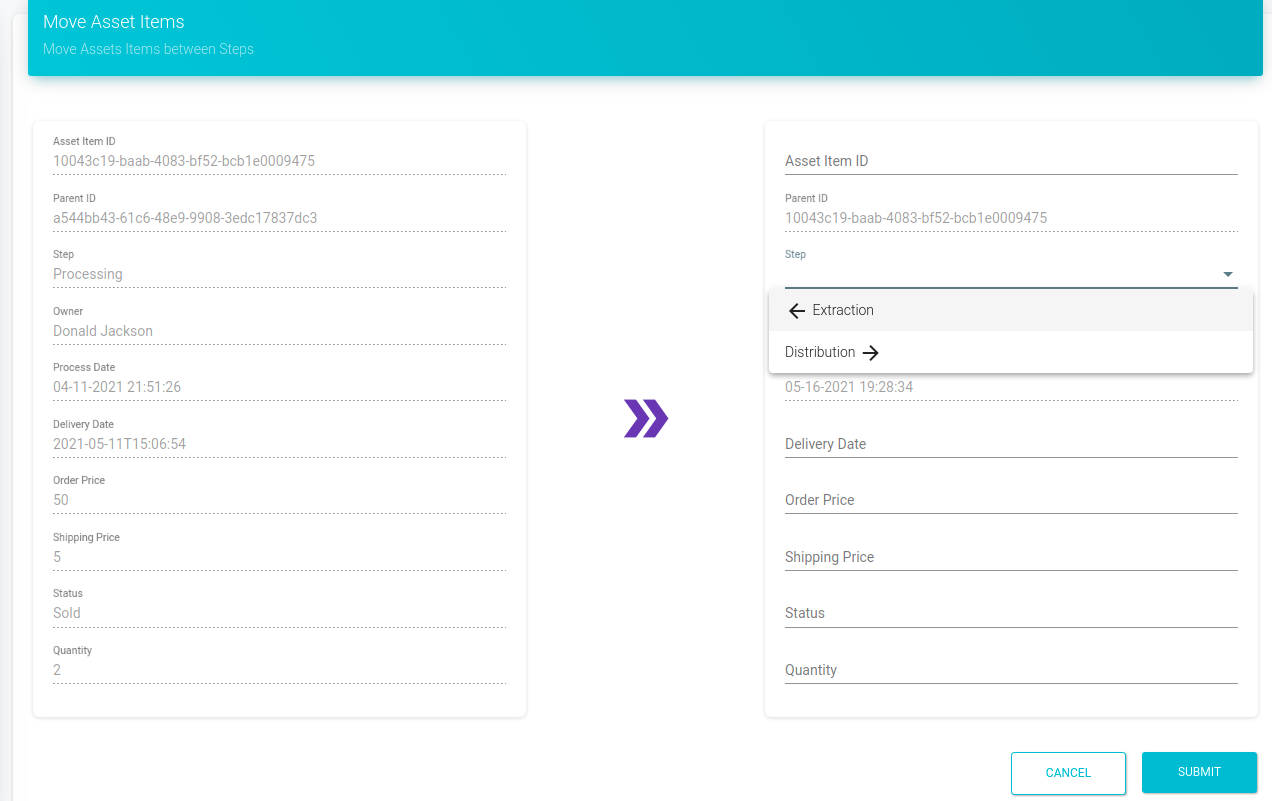
\includegraphics[scale=0.32]{images/use_example/091_move_asset_Item.png}
\caption{Move asset item form.}
\label{fig:move_asset_item}
\end{center}
\end{figure}

Track asset item displays the tracked info about the chosen asset item. It shows the children's tree of the selected element and its ancestors. Figure~\ref{fig:track_asset_item} shows the current status of the scenario described above by viewing the first asset item selected (the extracted coffee crop).

When clicking on a node in the chart, the information about the selected node is displayed under the diagram. Using this feature, the final user can track and see back that its cup of coffee has been passed. This information would be essential if a problem occurred. All the companies involved in this process could also track this information to understand better what happened, identify the possible step where a problem arose, and provide input for decision making.

\begin{figure}[H]
\begin{center}
  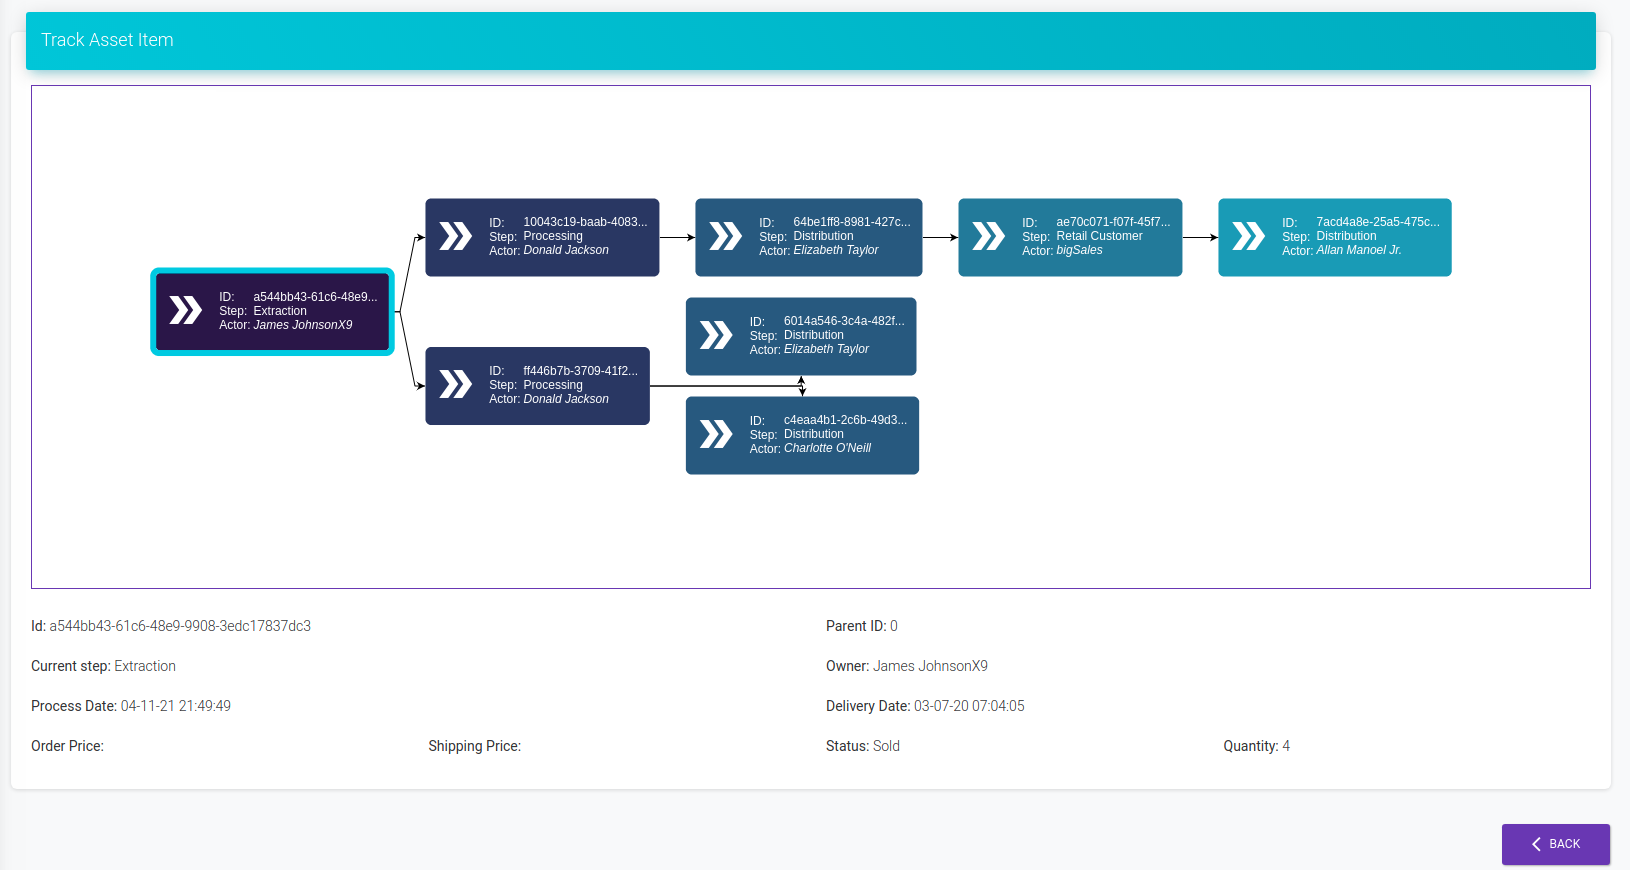
\includegraphics[scale=0.275]{images/use_example/092_track_asset_Item.png}
\caption{Track an asset item forward.}
\label{fig:track_asset_item}
\end{center}
\end{figure}


\begin{figure}[H]
\begin{center}
  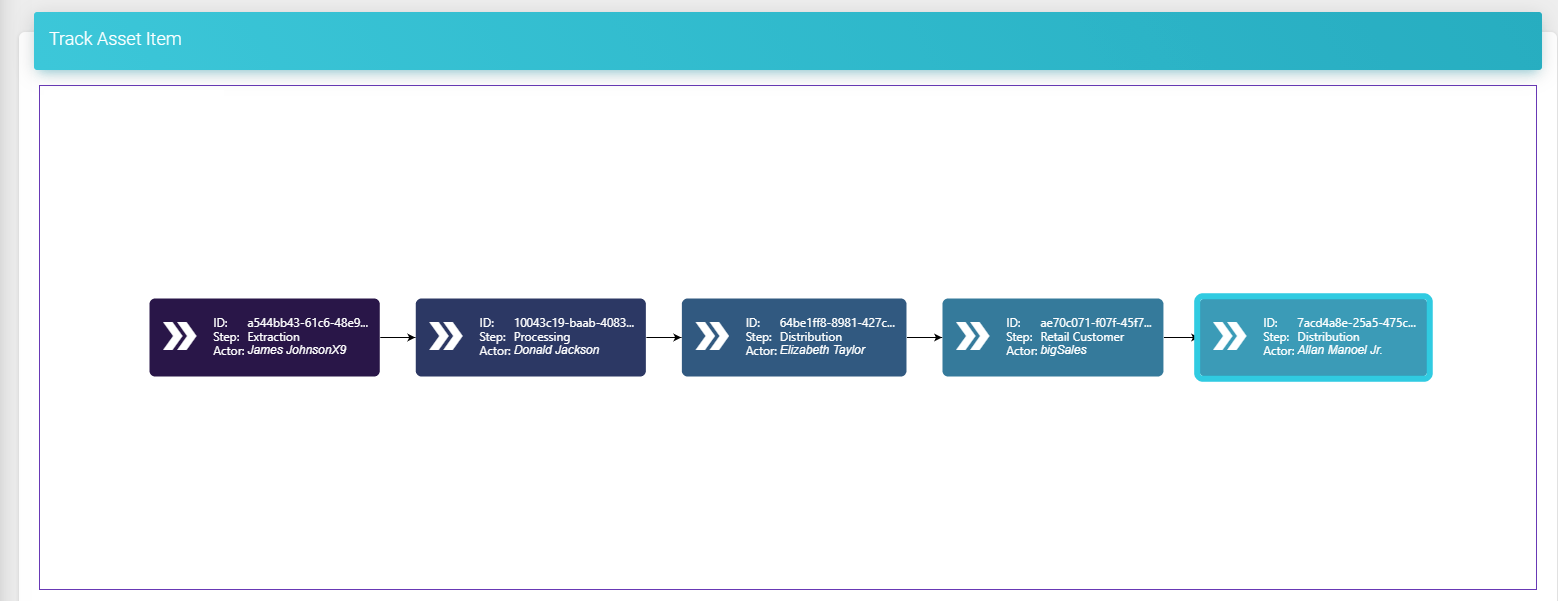
\includegraphics[scale=0.375]{images/use_example/trackbackwards.png}
\caption{Track an asset item backward.}
\label{fig:track_asset_item}
\end{center}
\end{figure}

Usage of blockchain helped to solve the problem since all the information under the blockchain is immutable. It can be audited since the information is stored and cannot be modified or deleted. The system allows anyone to check the previous' records traceability, which can be achieved by arriving at the beginning of the chain. A blockchain does play a key role in traceability, as it ensures the data logged is not tampered with once it has been saved to the blockchain.
 
 
 
 
 
%%\section{Steps and Substeps}\label{sec:stepsAndSubsteps}

%\subsection{Exploration}\label{sec:Exploration}
%Exploration is the starting point of a supply chain. Phase which encompasses Mineral Prospecting and Geological Survey.

%\subsubsection{Prospecting/ Surveying}\label{sec:Prospecting}
%Prospecting means the search of mineral occurrences/surveying means the research on a mineralised area, previously defined during the prospecting phase to be applied as a Mineral Right from the Mining Authority.

%\subsubsection{Mining right application}\label{sec:Mining}
%Through handing over documents to the Mining Authority (in Brazil it is Agência Nacional de Mineração [ANM]).

%\subsubsection{Geological Survey}\label{sec:GeologicalSurvey}
%Geological Survey is a set of activities carried out to determine the features on quality and quantity of ore found in a given mineral deposit.

%\subsubsection{Mineral reserve definition}\label{sec:MineralReserve}
%this step is related to the quantity of ore found during the Geological Survey.

%\subsection{Mine Development and Design}\label{sec:MineDevelopment}
%In this phase is made the preparation of a deposit to become a mine, opening accesses, setting up fences, building benches.


%\subsection{Production}\label{sec:Production}
%Production phase including ore extraction and mineral processing or transformation.

%\subsubsection{Quarrying/ Blasting plan}\label{sec:Quarrying}
%Quantity of stone extracted, same quantity of mineral reserves depleted, type of stone extracted.

%\subsubsection{Processing}\label{sec:Processing}
%Quantity of stone crushed/processed, same quantity of stone in stock deducted, type of stone product, market requirements.

%\subsubsection{Aggregate Product}\label{sec:AggregateProduct}
%Listing of products with identified quantities and respective technological features.

%\subsection{Distribution}\label{sec:Distribution}
%Product distribution with identification of clients and their segmentation. 

%\subsubsection{Client by Product Type}\label{sec:Client}
%Name, address, size, sector, business registration numbers (federal, state, municipal, county).

%\subsubsection{Transport}\label{sec:Transport}
%Invoice, bills, type of transportation, weight, distance.

%\subsection{Mine Closure}\label{sec:MineClosure}
%Mine Closure or mineral decommissioning, it means the end of the mining activity and the start of the installations removal and area remodelling through plantation and/or building a lake.

%\subsubsection{Legal Compliance/Decommissioning Plan}\label{sec:LegalCompliance}
%Status of all documentation related to the Decommissioning Plan and its Legal Compliance.

%\subsubsection{Environmental Recovery/ ANM %Application}\label{sec:EnvironmentalRecovery}
%Application number and status.

%\section{Target Goals}\label{sec:targetGoals}

These are goals for completing specific objectives:

\begin{enumerate}

\item Conduct functional requirements survey. Deadline: 01/06/2019 a 25/06/2019.
\begin{enumerate}
\item Develop application domain understanding;
\item Interact with stakeholders to gather requirements;
\item Classify requirements;
\item Set Requirements Priorities;
\end{enumerate}
\item Design system architecture. Deadline: 26/06/2019 a 25/07/2019.
\begin{enumerate}
\item Define key system modules and components;
\item Establish methods of interaction between components;
\item Make UML Component Diagram;
\item Make use-case UML diagram;
\item Create UML Activity Diagram;
\item Model data structure.
\end{enumerate}
\item Develop Web Application. Deadline: 26/07/2019 a 31/12/2019.
\begin{enumerate}
\item Implement back-end components;
\item Implement front-end components
\end{enumerate}
\item Develop smart contract. Deadline: 05/01/2020 a 29/02/2020.
\begin{enumerate}
\item Implement the chaincode;
\end{enumerate}
\item Perform system validations. Deadline: 01/03/2020 a 30/05/2020.
\begin{enumerate}
\item Perform functional tests;
\item Perform integration tests;
\item Perform security tests;
\item Create acceptance report based on \acf{TAM}.
\end{enumerate}
\end{enumerate}
%\section{Scientific Method}\label{sec:method}

For project development, the agile Scrum method has been used. In Scrum, projects are divided into cycles called sprints, with frequent meetings where the team can inform what is being done and think of ways to quickly improve the process. Scrum proposes constant project monitoring. Often the team will be meeting, exchanging experiences, evaluating what has been done and re-planning what will be done next.

During the requirements gathering, developers and other stakeholders sought to raise and prioritize the needs of future software users (referred as requirements). After the requirements gathering, in the requirements specification stage, developers made a detailed study of data collected in the previous activity, from where models were built to represent the software system being developed.

At the architectural design stage of the system two basic activities were performed: architectural design (or high level design), and detailed design (or low level design). Some aspects were considered at this stage of system design, such as: system architecture, platform used, Database Manager System (DBMS) used and graphical interface standard.

In the application development period, the backend and frontend components will be created from the computational description of the design phase. Pre-existing software tools and class libraries will be used to streamline the activity. These tools and libraries will be defined during the architectural design.

For system validation, two main requirements will be evaluated: the components and the behavior of who will use the application. For the first point, functional, integration and security tests will be performed. For the second, the \acf{TAM} method will be used to evaluate user acceptance, utility and ease of use.

The appendix \ref{app:projectManagement} presents the activities for project management, the user stories and non-functional requirements.